\section{Evaluation}
The purpose of selective decoding is to achieve more efficient zoomable video playback. We evaluate the efficiency of selective decoding from two aspects, video playback frame rate and energy consumption. 

We used a Samsung Galaxy S2 phone for experiment. The device has a dual core processor of 1200 MHz clock rate each and 1024 MB RAM, with Android 2.3.6 running. Two videos of 1080p are used for evaluation, one having little motion while the other containing constant object motion. We refer them as video A and video B respectively. 

\subsection{Frame Rate}
Selective video playback frame rate is affected by both ROI size and position. We designed experiments to examine the influence of each. 

\subsubsection{Different ROI Positions}
Different regions of a video frame may contain different amount of motions and dependencies, therefore the ROI position can affect the amount of processing at decoding and subsequently the video playback frame rate. We fix the ROI size, and then move the ROI from the upper left corner to the lower right of the video frame. The tests are repeated for three different ROI sizes, with the ROI width and height set as 50\%, 70\%, and 90\% of the original video's width and height. 

\begin{figure}
\centering
%\subfigure[Phone A Video 1]{\includegraphics[height=4.0cm]{fr1a1.eps}}
%\subfigure[Phone A Video 2]{\includegraphics[height=4.0cm]{fr1a2.eps}}
%\
\subfigure[Video A]{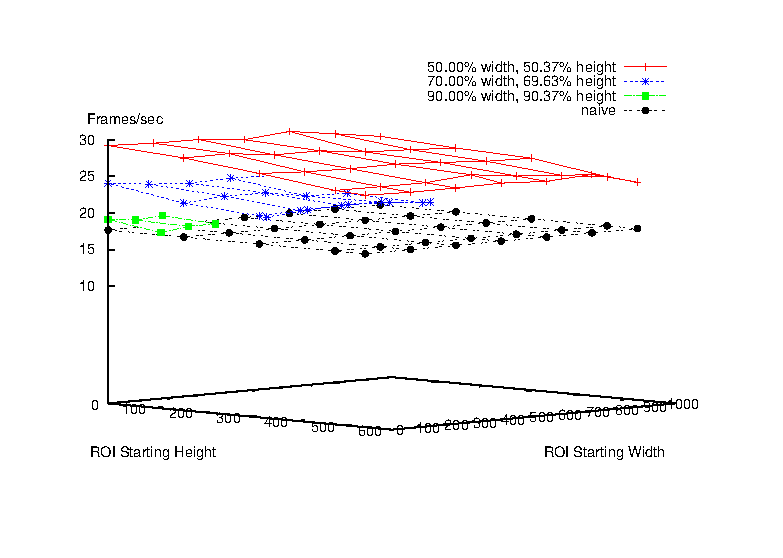
\includegraphics[height=4.0cm]{fr1b1.eps}}
\subfigure[Video B]{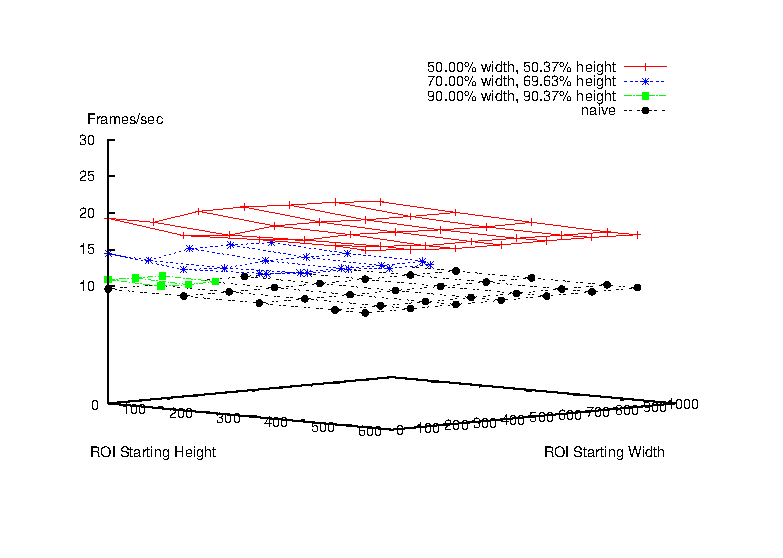
\includegraphics[height=4.0cm]{fr1b2.eps}}
\caption{Frame Rate with 90\%, 70\%, and 50\% of ROI at Different Positions}
\end{figure}
In Fig 8, each 3D interface indicates the frame rate for a ROI size. The intersection in a surface indicates the start position of a particular ROI size. 

Looking at each 3D interface, the frame rate tends to decrease when ROI starting width and/or starting height increases. This is because the intra-frame dependencies increase towards the lower right, and more dependencies cause more macroblocks to be selected and decoded. However, there are exceptions to this decrease trend, which are probably caused by different amount of motions at different ROI positions. Compare different 3D interfaces at a single figure, it is clear that the ROI size has a more significant effect than ROI position and selective decoding outperforms standard decoding. Compare Fig 8(a) with (b), the frame rate for video A is higher than video B. This is expected because video A has less amount of motion than video B. 

\subsubsection{Different ROI Size}
Previous experiment already reveals that ROI size has significant influence on video playback frame rate. This experiment examines the affection of ROI size further. We position the ROI at the center of the video frame and vary the ROI height and width from 10\% to 100\% of original video height and width.

\begin{figure}
\centering
%\subfigure[Phone A Video 1]{\includegraphics[height=2.0cm]{fr2a1.eps}}
%\subfigure[Phone A Video 2]{\includegraphics[height=2.0cm]{fr2a2.eps}}
\subfigure[Video A]{\includegraphics[height=3.0cm]{fr2b1.eps}}
\subfigure[Video B]{\includegraphics[height=3.0cm]{fr2b2.eps}}
\caption{Frame Rate with 10\% to 100\% ROI Centered}
\end{figure} 
Looking at either Fig 9(a) or (b), frame rate decreases as ROI size increases. Selective decoding achieves higher frame rate at ROI size smaller than 90\%. At 10\% ROI, the frame rate is improved by 76.3\% and 193.3\% for video A and B respectively. The curves at different figures differ due to different amount of motion at center of the video frame. 

%In addition to the two experiments above, we measured the overhead of selective decoding by setting the ROI as the entire frame. The overhead are 4.87\% and 1.34\% for video A and B respectively. In practice, we can switch between selective decoding and standard decoding dynamically based on ROI sizes to achieve higher frame rate. 
 
\subsection{Energy Consumption} 
Energy consumption is the other important aspect of our evaluation. Two experiments are done with different focuses.

\subsubsection{PowerTutor Measurements}
Battery energy is mainly consumed by display and CPU at video playback. PowerTutor\cite{Zhang:2010:AOP:1878961.1878982}, an Android power measurement tool, is capable of measuring power consumed by different hardware components for a user specified app. In this experiment, we vary ROI size from 10\% to 100\%. The frame rate is controlled so that both selective decoding and standard decoding always play at same rate. This is essential for a fair comparison because the CPU display power is dependent on display time. 

For display measurements, we found selective decoding and standard decoding consume almost same amount of energy. However, this is not the case for CPU power consumption, which is shown as Fig 10.
 
\begin{figure}
\centering
%\subfigure[Phone A Video 1]{\includegraphics[height=2.0cm]{pta1.eps}}
%\subfigure[Phone A Video 2]{\includegraphics[height=2.0cm]{pta2.eps}}
\subfigure[Video A]{\includegraphics[height=3.0cm]{ptb1.eps}}
\subfigure[Video B]{\includegraphics[height=3.0cm]{ptb2.eps}}
\caption{CPU Power Consumption Per Frame}
\end{figure}
Looking at each figure individually, CPU power consumption per frame at selective decoding increases when ROI size increases. At ROI size 90\% or less, selective decoding consumes less CPU energy than standard decoding. Compare Fig 10(a) with (b), video playback for heavy motion video tends to consume more power because of more motion compensation decoding. 

\subsubsection{Power Drain Experiment}
PowerTutor measurements show selective decoding can save energy, mainly by reducing CPU power consumption. However, PowerTutor measurement is obtained through offline-training models\cite{Zhang:2010:AOP:1878961.1878982} and may not be accurate for all phones. We designed another experiment to measure the power consumption. 

\begin{figure}
\centering
%\subfigure[Phone A Video 1]{\includegraphics[height=2.0cm]{pwa1.eps}}
%\subfigure[Phone A Video 2]{\includegraphics[height=2.0cm]{pwa2.eps}}
\subfigure[Video A]{\includegraphics[height=3.0cm]{pwb1.eps}}
\subfigure[Video B]{\includegraphics[height=3.0cm]{pwb2.eps}}
\caption{Percentage of Power Drained}
\end{figure}
In this experiment, we place ROI at the video frame center and play the video repeatedly with constant frame rate. Based on the processing power and video, we set the frame rate for two videos as 15 FPS and 8FPS respectively. The percentage of power drained is recorded for comparison. Before each test, we fully charge the phone battery to 100\% and disable all background activities including Wi-Fi, Bluetooth, GPS, etc.

Looking at each figure individually, selective decoding consumes less power. At 10\% ROI size, the battery consumption is reduced by 61.1\% and 64.5\%. Because we set the frame rate differently for videos, the comparison for different videos is not fair and therefore avoided.  

In summary, selective decoding proves to be efficient in terms of playback frame rate and battery energy consumption when ROI size is below certain threshold.  




